% !Mode:: "TeX:UTF-8"
%!TEX program  = xelatex

% \documentclass{cumcmthesis}
\documentclass[withoutpreface,bwprint]{cumcmthesis} %去掉封面与编号页

\usepackage{url}
\title{Analysis and Forecast of the Pet Industry through Mathematical Models}
% \tihao{A}
% \baominghao{4321}
% \schoolname{XX大学}
% \membera{小米}
% \memberb{向左}
% \memberc{哈哈}
% \supervisor{老师}
% \yearinput{2017}
% \monthinput{08}
% \dayinput{22}
\usepackage{ctex}
\usepackage{setspace}
\usepackage{lipsum}
\usepackage{graphicx}%插入图片
\usepackage{cite}
\usepackage{hyperref}
\begin{document}
\bibliographystyle{plain}% 参考文献引用格式
 \maketitle
 \begin{abstract}
    The pet industry has witnessed significant growth globally, driven by increasing disposable income and the rising popularity of pet companionship. This paper explores the development and forecasting of the pet industry using mathematical models, with a focus on China's market trends and global demands. Through the application of ARIMA, polynomial interpolation, and multiple linear regression, this study analyzes the past five years of the pet industry in China, forecasting its development over the next three years. Additionally, global trends and the impact of economic factors, such as tariffs, on the pet food industry are considered. The results provide valuable insights for strategic recommendations and sustainable development in the pet industry.
    
% \uwave{关注我们的微信公众号}:
\begin{figure}[htbp]
	\centering
	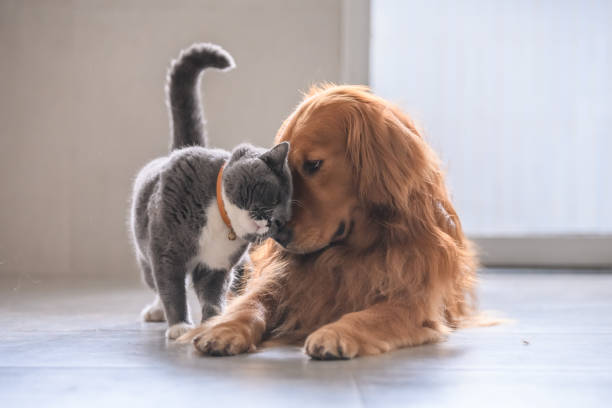
\includegraphics[scale=2.5]{istockphoto-992637094-612x612}
	\caption{British short hair cat and golden retriever stock photo\cite{1}}
\end{figure}
% \centerline{
\includegraphics[width=5cm]{gongzhonghao}}
% \caption{this is Ali}

\keywords{Pet Industry, Mathematical Models, ARIMA, Polynomial Interpolation, Multiple Linear Regression, Forecasting, Market Analysis, Economic Factors, Pet Food, Sustainable Development}
\end{abstract}

%目录
\tableofcontents

\section{Problem Restatement}

This problem requires analyzing and forecasting the development trends of the pet industry in China and globally, with a focus on the pet food market. The analysis should combine historical data and additional data collected, building mathematical models for prediction. The specific tasks are as follows:
\subsection{Question 1: Development of China's Pet Industry}

\subsubsection{Objective}
Analyze the development of China's pet industry over the past five years by different pet types (e.g., cats, dogs, etc.).
\subsubsection{Factors}
Look into economic factors, societal trends, and market changes (e.g., income growth, changes in pet ownership behavior, product innovations).
\subsubsection{Modeling Task}
Develop a mathematical model to predict the growth and development of China's pet industry for the next three years.
\subsection{Question 2: Global Pet Industry Development}
\subsubsection{Objective}
Analyze the development of the global pet industry, focusing on different regions (e.g., Europe, America, China).
\subsubsection{Factors}
Global pet food demand and market characteristics by pet type.
\subsubsection{Modeling Task}
Create a model to forecast the global demand for pet food over the next three years, based on data provided.
\subsection{Question 3: China's Pet Food Industry}
\subsubsection{Objective}
Analyze the development of China's pet food industry, specifically its production and export values.
\subsubsection{Factors}
The trend in China's pet food production and exports, factoring in the global demand for pet food.
\subsubsection{Modeling Task}
Predict China's pet food production and export trends over the next three years.
\subsection{Question 4: Impact of Foreign Economic Policies}
\subsubsection{Objective}
Analyze the impact of foreign economic policies on China's pet industry, focusing on trade barriers and tariffs.
\subsubsection{Factors}
Quantitative modeling of the effects of changes in tariffs and other foreign policies on China's pet food industry.
\subsubsection{Modeling Task}
Develop a model to assess the impact of these policies on China's pet food industry and suggest strategies for sustainable development.
\section{Model Assumptions}

\begin{itemize}
    \item Stability of human society
    \item Exclusion of potential future policies related to pets
    \item Ignoring changes in pet population due to major incidents
\end{itemize}

\section{Symbol Explanation}
\begin{center}
\begin{tabular}{cc}
 \hline
 \makebox[0.3\textwidth][c]{Symbol}	&  \makebox[0.4\textwidth][c]{Meaning} \\ \hline
 $\ln$ 	    & Logarithmic Function \\ \hline
 $\sum$ 	    & Sum  \\ \hline
 $M$	    & Million  \\ \hline
 $N$	    & Number  \\ \hline
\end{tabular}
\end{center}

\section{Analysis}

\subsection{Question 1 Analysis}
\subsubsection{Analyze factors}
The task first requires us to analyze the development trends of the pet industry in China by categorizing pets 
and identifying the factors that influence the growth of the pet industry.
We should begin by analyzing the data.
\par The following data is provided to us in the problem.
\begin{table}[!htbp]
    \caption{2019-2023 Number of Pet Cats and Dogs in China (in 10,000s)} \centering
    \begin{tabular}{cccccc}
    \toprule[1.5pt]
    Pets/Years & 2023 & 2022 & 2021 & 2020 & 2019 \\
    \midrule[1pt]
    Cat & 6980 & 6536 & 5806 & 4862 & 4412 \\
    Dog & 5175 & 5119 & 5429 & 5222 & 5503 \\
    \bottomrule[1.5pt]
    \end{tabular}
    \end{table}
\par Plot the trend of changes in the pet population in China. 
A line chart is more intuitive than a table.
Thanks to the help of python, we can easily plot the line chart by the following code.
\begin{lstlisting}[language=python]
import pandas as pd
import matplotlib.pyplot as plt
with open('data_1.txt', 'r') as file:
    lines = file.readlines()
years = lines[0].split()[1:]
cat_data = lines[1].split()[1:]
dog_data = lines[2].split()[1:]
years = [int(year) for year in years]
cat_data = [int(num) for num in cat_data]
dog_data = [int(num) for num in dog_data]
plt.figure(figsize=(10, 6))
plt.plot(years, cat_data, marker='o', label='Cat')
plt.plot(years, dog_data, marker='o', label='Dog')
plt.xlabel('Year')
plt.ylabel('Number')
plt.title('Cat and Dog Numbers Over Years')
plt.legend()
plt.grid(True)
plt.show()
\end{lstlisting}
\begin{figure}[htbp]
	\centering
	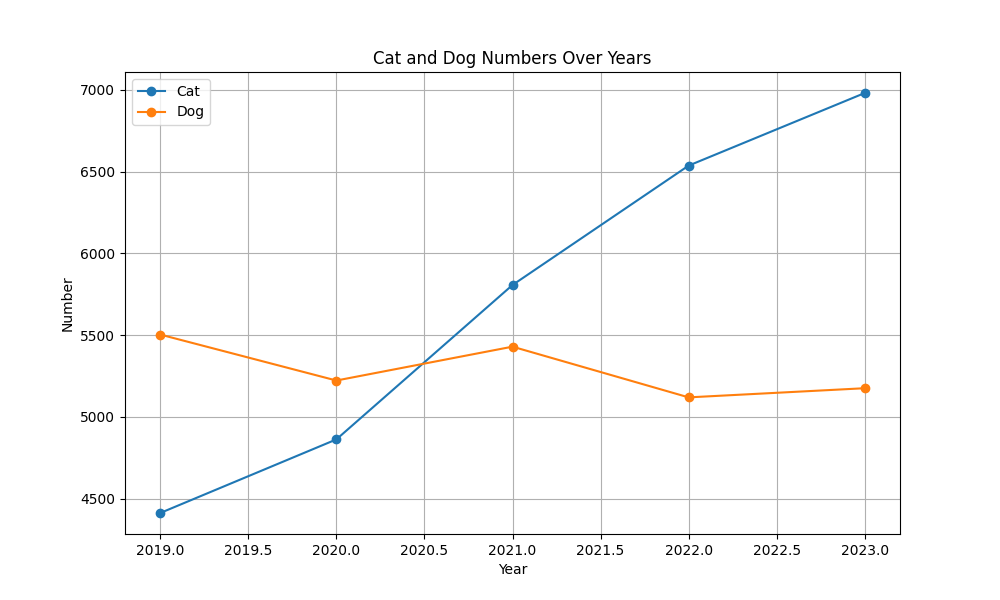
\includegraphics[scale=0.6]{Figure_2}
	\caption{Number of Cat and Dog in China from 2019 to 2023}
\end{figure}
\par From the graph, we can see that the number of cats is increasing, while the number of dogs remains almost unchanged. This growth in the cat population is likely due to the improvement in living standards, with more and more people beginning to keep pets.
Therefore, GDP is likely one of the factors influencing the pet population. By reviewing relevant data, we found a strong correlation between the growth rate of GDP and the growth rate of the pet population.
Thus, to predict the growth of the pet population, we can use the growth rate of GDP as an indicator.
As for dogs, we did not find a direct relationship between the GDP growth rate and the growth rate of the dog population. However, we can be certain that the development of the pet economy will drive the growth of the pet population.
Hence, the pet economy is likely to have a strong correlation with the growth of the pet population.
\par Summarizing the above analysis, we assume that the growth of the pet population is influenced by the growth rate of GDP.
\subsubsection{Polynomial Interpolation}
\par We aim to predict the data for the next three years based on the data from the previous five years, starting with polynomial interpolation.
\begin{definition}[Polynomial Interpolation]
Given \( n+1 \) points, polynomial interpolation refers to finding a polynomial such that it satisfies the condition
\[
    P(x) = a_n x^n + a_{n-1} x^{n-1} + \dots + a_1 x + a_0
\]
That is, the image of the polynomial \( y = P(x) \) must pass through the given \( n+1 \) points \( (x_i, y_i) \).
\end{definition}
\par Because \( P(x) \) can pass through these existing points and \( P(x) \) is a polynomial, \( P(x) \) may indeed reflect the trend of data changes to some extent.
\par We tried simple polynomial interpolation, with time as the independent variable and the number of cats and dogs as the dependent variable, to perform polynomial interpolation.
\begin{lstlisting}[language=python]
for n in range(1, 10):
    coeffs_cat = np.polyfit(years, cat_data, n)
    coeffs_dog = np.polyfit(years, dog_data, n)
    y_poly_pred_cat = np.polyval(coeffs_cat, years)
    y_poly_pred_dog = np.polyval(coeffs_dog, years)
    new_x = np.array([2019, 2020, 2021, 2022, 2023, 2024, 2025, 2026])
    new_y_cat = np.polyval(coeffs_cat, new_x)
    new_y_dog = np.polyval(coeffs_dog, new_x)
    plt.figure(figsize=(10, 6))
    plt.plot(years, cat_data, marker='o', label='Cat')
    plt.plot(years, dog_data, marker='o', label='Dog')
\end{lstlisting}
\par Define \( k \) as the degree of the polynomial, \( n \) as the number of points, when \( k >= n \), Function polyfit can be considered as(in fact not because of simplicity) using Lagrange interpolation to perform polynomial interpolation.
\begin{definition}[Lagrange Interpolation]
    Given a set of distinct nodes \( x_0, x_1, \dots, x_n \) and the corresponding function values \( y_0, y_1, \dots, y_n \), the Lagrange interpolation polynomial \( L(x) \) is the polynomial that interpolates these points, defined as:

    \[
    L(x) = \sum_{i=0}^{n} y_i \ell_i(x)
    \]
    
    where \( \ell_i(x) \) is the \( i \)-th Lagrange basis polynomial, defined as:
    
    \[
    \ell_i(x) = \prod_{\substack{0 \leq j \leq n \\ j \neq i}} \frac{x - x_j}{x_i - x_j}
    \]
    
    This polynomial satisfies: \( \ell_i(x_j) = \delta_{ij} \), where \( \delta_{ij} \) is the Kronecker delta, which is 1 when \( i = j \) and 0 otherwise.
    
\end{definition}
\par The following is the result of the polynomial interpolation.
\clearpage
\begin{figure}[htbp]
	\centering
	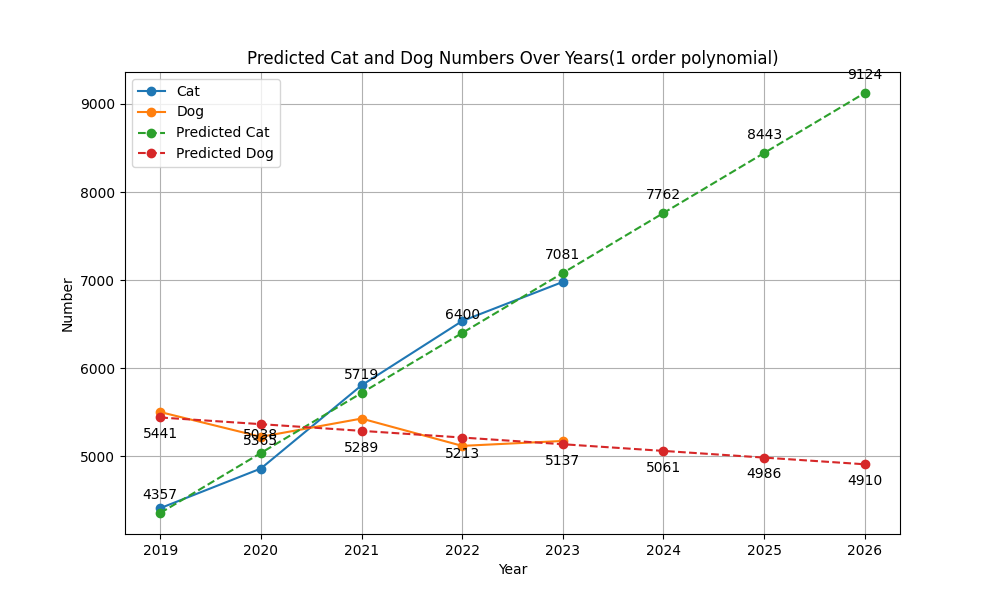
\includegraphics[width=.99\textwidth]{q1_1}
	\caption{Linear Interpolation of Cat and Dog Numbers}
\end{figure}
\par We can find that although it is linear interpolation, the fitting effect is already very good.
However, when the degree of the polynomial is increased, the fitting effect is not significantly improved.
And because we only have five points, when the degree of the polynomial is greater than 5, the fitting effect is actually worse.
To solve the above problems and apply the two influencing factors mentioned earlier, we use the following model.
Its core idea is also fitting, but it is a higher dimension fitting.
Its essence has not changed, but the number of independent variables has increased.
\par First, we collected the relevant data.
% years 2023 2022 2021 2020 2019
% GDP 12614 12662 12617 10408 10143
\begin{table}[!htbp]
    \caption{2019-2023 GDP in China (in 10 billion yuan)\cite{2}} \centering
    \begin{tabular}{cccccc}
    \toprule[1.5pt]
    Years & 2023 & 2022 & 2021 & 2020 & 2019 \\
    \midrule[1pt]
    GDP & 12614 & 12662 & 12617 & 10408 & 10143 \\
    \bottomrule[1.5pt]
    \end{tabular}
\end{table}
% years 2023 2022 2021 2020 2019
% pet_industry_economy 3264 3069 2733 2259 2191
\begin{table}[!htbp]
    \caption{2019-2023 Pet Industry Economy in China (in 100 million yuan)\cite{3}} \centering
    \begin{tabular}{cccccc}
    \toprule[1.5pt]
    Years & 2023 & 2022 & 2021 & 2020 & 2019 \\
    \midrule[1pt]
    Pet Industry Economy & 3264 & 3069 & 2733 & 2259 & 2191 \\
    \bottomrule[1.5pt]
    \end{tabular}
\end{table}
\begin{figure}[htbp]
	\centering
	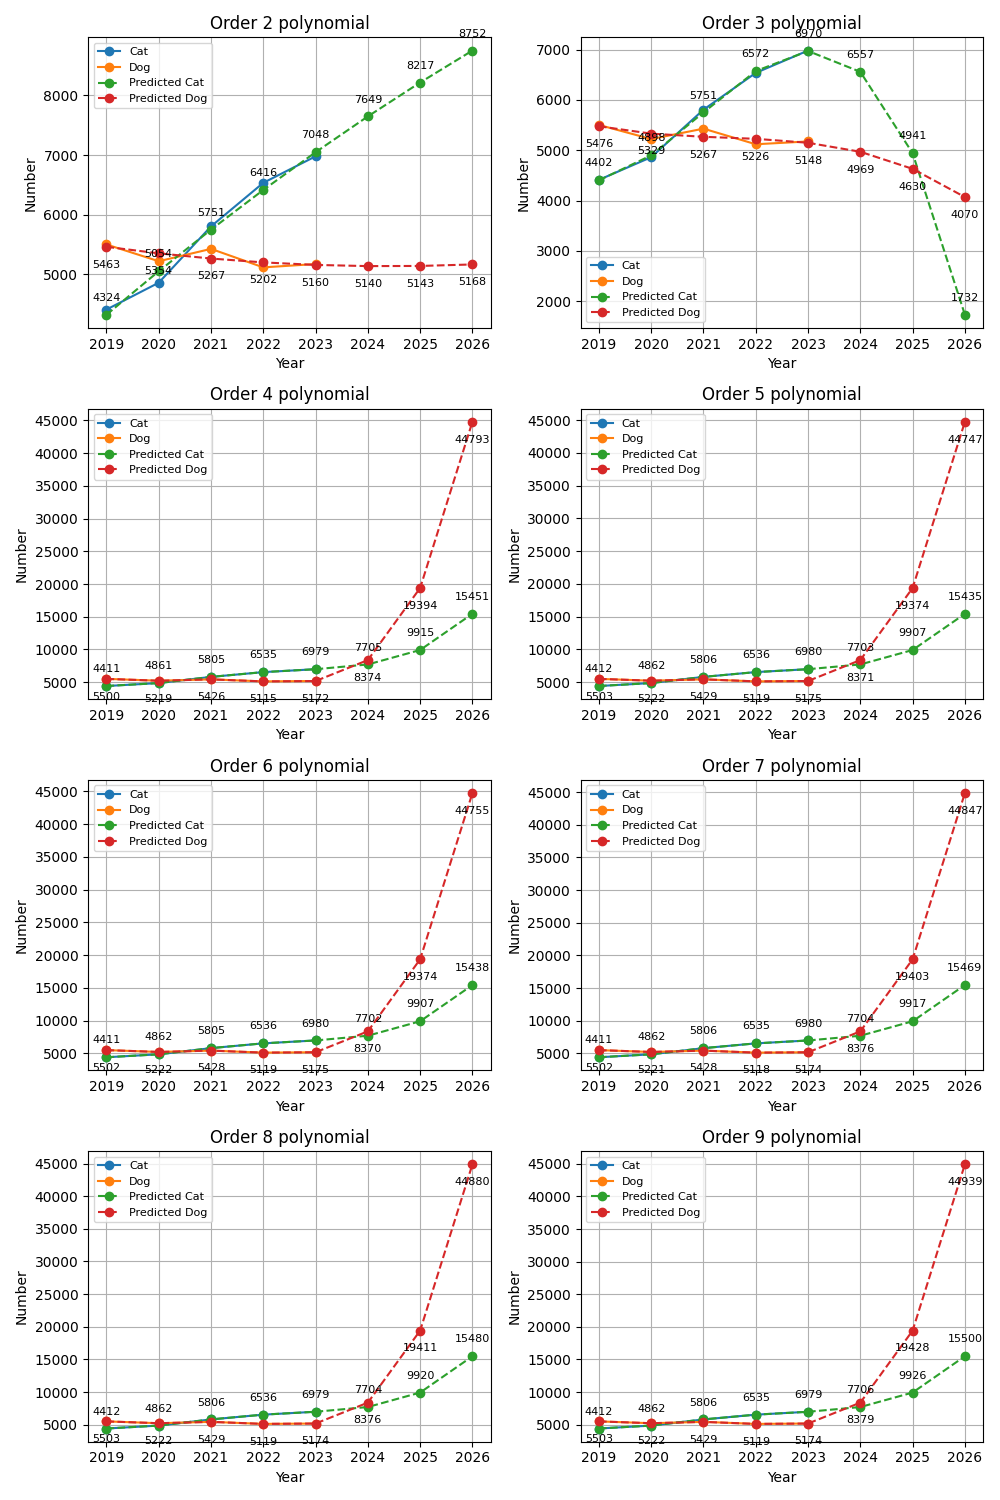
\includegraphics[width=.99\textwidth]{q1_all}
	\caption{Polynomial Interpolation of Cat and Dog Numbers}
\end{figure}
\clearpage
\subsubsection{Multiple Linear Regression}
\par Similarly, in three-dimensional space, we can also find a plane that fits all the points.
\begin{figure}[htbp]
	\centering
	\includegraphics[width=.85\textwidth]{figure_4}
	\caption{Three-Dimensional Polynomial Interpolation of Pet Economy-Year-Pets}
\end{figure}
\begin{figure}[htbp]
	\centering
	\includegraphics[width=.85\textwidth]{figure_5}
	\caption{Three-Dimensional Polynomial Interpolation of GDP-Year-Pets}
\end{figure}
\begin{definition}[Multiple Linear Regression]
Multiple Linear Regression is a statistical method used to model the relationship between two or more independent variables and a dependent variable. Suppose we have a dataset consisting of $n$ data points, each with $m$ independent variables and one dependent variable. The goal is to find the best-fitting hyperplane that describes the relationship between the independent and dependent variables.
\end{definition}

\begin{solution}
Assume we have $n$ observations, each with $m$ features. Each observation can be represented as:
\[
\mathbf{x}_i = (x_{i1}, x_{i2}, \dots, x_{im})^T, \quad y_i
\]
where $y_i$ is the dependent variable for the $i$-th observation, and $\mathbf{x}_i$ is the corresponding independent variable vector. Our goal is to fit the multiple linear regression model to the following equation:
\[
y_i = \beta_0 + \beta_1 x_{i1} + \beta_2 x_{i2} + \dots + \beta_m x_{im} + \epsilon_i
\]
where $\beta_0$ is the intercept term, $\beta_1, \beta_2, \dots, \beta_m$ are the regression coefficients, and $\epsilon_i$ is the error term, assumed to have zero mean and constant variance.


Let us represent all observations in matrix form. Suppose we have $n$ data points, each with $m$ features, the data can be written as:
\[
\mathbf{X} = \begin{pmatrix}
1 & x_{11} & x_{12} & \dots & x_{1m} \\
1 & x_{21} & x_{22} & \dots & x_{2m} \\
\vdots & \vdots & \vdots & \ddots & \vdots \\
1 & x_{n1} & x_{n2} & \dots & x_{nm}
\end{pmatrix}
\]
\[
\mathbf{y} = \begin{pmatrix}
y_1 \\
y_2 \\
\vdots \\
y_n
\end{pmatrix}
\]
where $\mathbf{X}$ is an $n \times (m+1)$ design matrix with the first column as ones, and $\mathbf{y}$ is an $n \times 1$ vector of the dependent variables.

The regression coefficients $\boldsymbol{\beta}$ are given by:
\[
\boldsymbol{\beta} = \begin{pmatrix}
\beta_0 \\
\beta_1 \\
\vdots \\
\beta_m
\end{pmatrix}
\]

Thus, the regression model in matrix form is:
\[
\mathbf{y} = \mathbf{X} \boldsymbol{\beta} + \boldsymbol{\epsilon}
\]
where $\boldsymbol{\epsilon}$ is the vector of errors.
To estimate the regression coefficients $\boldsymbol{\beta}$, we minimize the residual sum of squares (RSS):
\[
RSS = \sum_{i=1}^{n} (y_i - \hat{y}_i)^2 = (\mathbf{y} - \mathbf{X} \boldsymbol{\beta})^T (\mathbf{y} - \mathbf{X} \boldsymbol{\beta})
\]
Taking the derivative with respect to $\boldsymbol{\beta}$ and setting it equal to zero, we obtain the normal equation:
\[
\mathbf{X}^T \mathbf{X} \boldsymbol{\beta} = \mathbf{X}^T \mathbf{y}
\]
Solving this equation gives the estimated regression coefficients:
\[
\boldsymbol{\beta} = (\mathbf{X}^T \mathbf{X})^{-1} \mathbf{X}^T \mathbf{y}
\]
\end{solution}
\begin{lstlisting}[language=python]
# key code
from sklearn.linear_model import LinearRegression
regressor_cat = LinearRegression()
regressor_cat.fit(X_cat, cat)
x_grid, y_grid = np.meshgrid(np.linspace(x.min(), x.max(), 30),
                                np.linspace(y.min(), y.max(), 30))
z_pred_cat = regressor_cat.predict(np.column_stack(
    (x_grid.ravel(), y_grid.ravel()))).reshape(x_grid.shape)
surf_cat = ax.plot_surface(
    x_grid, y_grid, z_pred_cat, alpha=0.3, cmap='Reds')
\end{lstlisting}
\par the problem is that we only have one independent variable, which is time,
and only one dimension of data, so we can't find the corresponding points on the plane.
we have to predict the data of GDP and pet industry economy 
so as to find the corresponding points on the plane.
One good way is to use the linear regression model.
\clearpage
\begin{figure}[htbp]
	\centering
	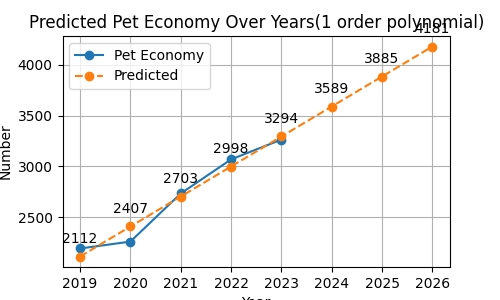
\includegraphics[width=.85\textwidth]{q3_1}
	\caption{Linear Regression of Pet Industry Economy-Year-Pets}
\end{figure}
\begin{figure}[htbp]
	\centering
	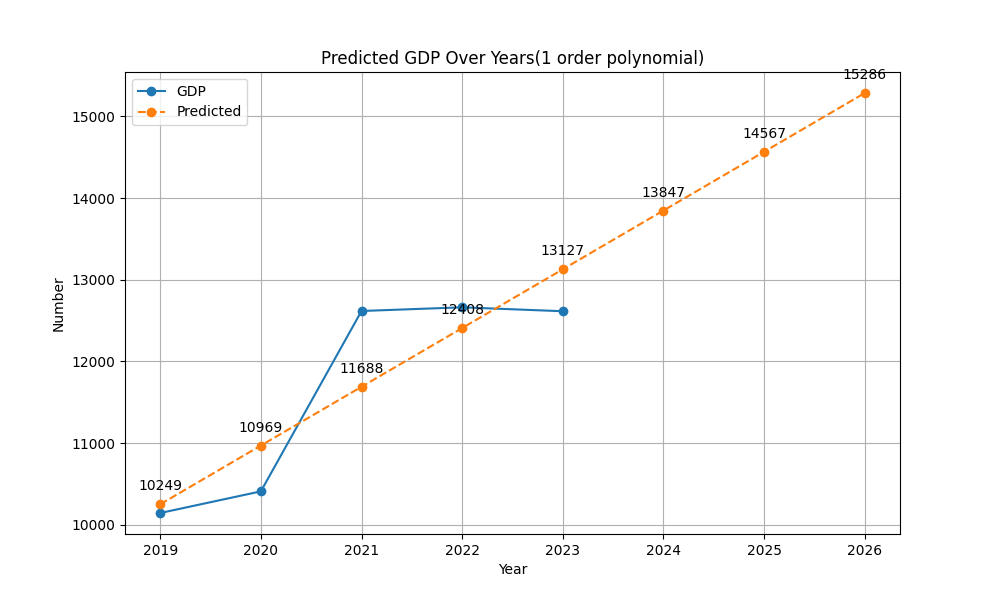
\includegraphics[width=.85\textwidth]{q2_1}
	\caption{Linear Regression of GDP-Year-Pets}
\end{figure}
\par We can see that the fitting effect is very good for pet industry economy.
But as for GDP, the fitting effect is a bit poor.It original data looks like a logarithm curve.
Using logarithm curve to fit the data, we can get a better fitting effect.
\begin{definition}[Logarithmic Curve Fitting]
The logarithmic model is expressed as:
\[
y = \sum_{i=0}^{n} a_i [\ln(bx + c)]^i = a_0 + a_1 \ln(bx + c) + a_2 [\ln(bx + c)]^2 + \dots + a_n [\ln(bx + c)]^n
\]
where \(a_i\), \(b\), and \(c\) are constants, and \(x\) and \(y\) are the data points.
\end{definition}
\begin{solution}
To fit the logarithmic curve, we can use the following procedure.
let \(z = \ln(bx + c)\), then the model becomes:
\[
y = \sum_{i=0}^{n} a_i z^i = a_0 + a_1 z + a_2 z^2 + \dots + a_n z^n
\]
which is a polynomial model, we can use the polynomial regression model to fit the data.
\end{solution}
\bibliography{books}




% \bigskip
% table环境是一个将表格嵌入文本的浮动环境。
% tabular环境的必选参数由每列对应一个格式字符所组成:c表示居中,l表示左对齐,r表示右对齐,其总
% 个数应与表的列数相同。此外,\verb|@{文本}|可以出现在任意两个上述的列格式之间,其中的文本将被插入每一行
% 的同一位置。表格的各行以\verb|\\|分隔,同一行的各列则以\&分隔。
% \verb|\toprule|、\verb|\midrule|和\verb|\bottomrule|三个命令是由booktabs宏包提供的,其
% 中\verb|\toprule|和\verb|\bottomrule|分别用来绘制表格的第一条(表格最顶部)和第三条(表格最底部)水平线,
% \verb|\midrule|用来绘制第二条(表头之下)水平线,且第一条和第三条水平线的线宽为1.5pt,第二条水平线的线宽为1pt。
% 引用方法:“如表~\verb|\ref{标签名}|~所示”。


% %参考文献
% \begin{thebibliography}{9}%宽度9
%  \bibitem{bib:one} ....
%  \bibitem{bib:two} ....
% \end{thebibliography}

% \newpage
% %附录
% \begin{appendices}
% \section{排队算法--matlab 源程序}
% \begin{lstlisting}[language=matlab]
% kk=2;[mdd,ndd]=size(dd);
% while ~isempty(V)
% [tmpd,j]=min(W(i,V));tmpj=V(j);
% for k=2:ndd
% [tmp1,jj]=min(dd(1,k)+W(dd(2,k),V));
% tmp2=V(jj);tt(k-1,:)=[tmp1,tmp2,jj];
% end
% tmp=[tmpd,tmpj,j;tt];[tmp3,tmp4]=min(tmp(:,1));
% if tmp3==tmpd, ss(1:2,kk)=[i;tmp(tmp4,2)];
% else,tmp5=find(ss(:,tmp4)~=0);tmp6=length(tmp5);
% if dd(2,tmp4)==ss(tmp6,tmp4)
% ss(1:tmp6+1,kk)=[ss(tmp5,tmp4);tmp(tmp4,2)];
% else, ss(1:3,kk)=[i;dd(2,tmp4);tmp(tmp4,2)];
% end;end
% dd=[dd,[tmp3;tmp(tmp4,2)]];V(tmp(tmp4,3))=[];
% [mdd,ndd]=size(dd);kk=kk+1;
% end; S=ss; D=dd(1,:);
%  \end{lstlisting}
%  \section{规划解决程序--lingo源代码}
% \begin{lstlisting}[language=c]
% kk=2;
% [mdd,ndd]=size(dd);
% while ~isempty(V)
%     [tmpd,j]=min(W(i,V));tmpj=V(j);
% for k=2:ndd
%     [tmp1,jj]=min(dd(1,k)+W(dd(2,k),V));
%     tmp2=V(jj);tt(k-1,:)=[tmp1,tmp2,jj];
% end
%     tmp=[tmpd,tmpj,j;tt];[tmp3,tmp4]=min(tmp(:,1));
% if tmp3==tmpd, ss(1:2,kk)=[i;tmp(tmp4,2)];
% else,tmp5=find(ss(:,tmp4)~=0);tmp6=length(tmp5);
% if dd(2,tmp4)==ss(tmp6,tmp4)
%     ss(1:tmp6+1,kk)=[ss(tmp5,tmp4);tmp(tmp4,2)];
% else, ss(1:3,kk)=[i;dd(2,tmp4);tmp(tmp4,2)];
% end;
% end
%     dd=[dd,[tmp3;tmp(tmp4,2)]];V(tmp(tmp4,3))=[];
%     [mdd,ndd]=size(dd);
%     kk=kk+1;
% end;
% S=ss;
% D=dd(1,:);
%  \end{lstlisting}
% \end{appendices}

\end{document} 